\section{Desarrollo del diseño} \label{sec:desarrollo-diseno}
En la Figura \ref{fig:metodologia} se puede visualizar la metodología que se llevó a cabo para cumplir con los objetivos previamente descritos. Se implementó una metodología similar a la metodología de \textit{benchmarking} ya que esta busca comparar el comportamiento de una empresa contra un estándar o el comportamiento de la mejor empresa. El propósito de esta metodología es encontrar las mejores prácticas disponibles, así como los aspectos por mejorar dentro de una empresa o un proceso específico de la empresa. Esta metodología implica definir métricas relevantes, recolección de información de diferentes fuentes y analizar dichas fuentes para identificar fortalezas y debilidades. En la metodología \textit{benchmark}, las métricas relevantes se denomina \textit{\acrlong{kpis}} (\acrshort{kpis}), los cuales son métricas específicas que juegan un rol crucial para determinar el nivel de la empresa comparada con el estándar o la mejor empresa. De igual manera, los \acrshort{kpis} también sirven para mostrarle a la empresa cuáles son las áreas por mejorar. La recolección y evaluación de fuentes, al igual que la determinación de los \acrshort{kpis}, son pasos cruciales para poder determinar el nivel correcto de la empresa. En especial, al seleccionar y evaluar las fuentes, se está construyendo un marco de referencias que contempla varias puntos de vista, nutridos de diferentes fuentes de información. En este proyecto en particular, el \textit{benchmarking} se utilizó para construir una estrategia que ayudará a las empresas a determinar su nivel de madurez en cuanto a conocimientos y acciones sobre las dependencias e impactos relacionados con el agua como capital natural. Adicionalmente, esta metodología también fue utilizada para determinar cuáles son los indicadores, relacionados al agua,  que se deberán evaluar o solicitar a las empresas. Esta paso fue solo aplicado en la estrategia solución, se hace esta distinción porque en las otras estrategias que fueron planteadas pero no ejecutadas la selección de indicadores no existía. 

\begin{figure}[H]
    \centering
    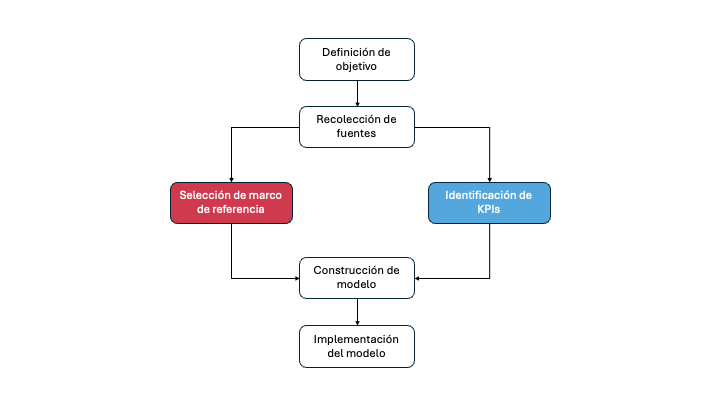
\includegraphics[scale=0.5]{images/4-desarrollo/diagrama-metodologia.png}
    \caption{Metodología utilizada}
    \label{fig:metodologia}
\end{figure}


En la Figura \ref{fig:estrategia} se presenta cual fue, además de la metodología previamente descrita, los componentes y el orden que se tuvieron en cuenta para cada estrategia. Cabe aclarar que no todas las estrategias planteadas contemplaban todos los componentes. Como se verá en la sección \ref{subsec:alternativas-diseno} \nameref{subsec:alternativas-diseno}, los motivos principales por los cuales se descartaron estrategias son por no considerar todos los componentes.  Los ‘Parámetros’ hacen referencia a parámetros que cada estrategia tuvo en cuenta. El primer parámetro, 'Concepto a evaluar', se refiere al componente del ecosistema que se evaluará. Algunos valores válidos pueden incluir ecosistema, servicios ecosistémicos, agua, carbono, especies, entre otros. El 'concepto a evaluar' es el aspecto sobre el cual la empresa está interesada en evaluar sus conocimientos y acciones, y del cual depende e impacta. El parámetro denominado 'Contexto de la empresa' se refiere al sujeto que será evaluado. Esto implica determinar si la estrategia se aplicará a una empresa específica o si se desarrollará para una empresa genérica. El último parámetro, ‘Granularidad empresarial’, se refiere a el nivel de la empresa que será evaluado. Por ejemplo, la granularidad más abstracta hace referencia a toda la empresa, mientras que la granularidad más precisa es un proceso en específico de la empresa. 

\begin{figure}[H]
    \centering
    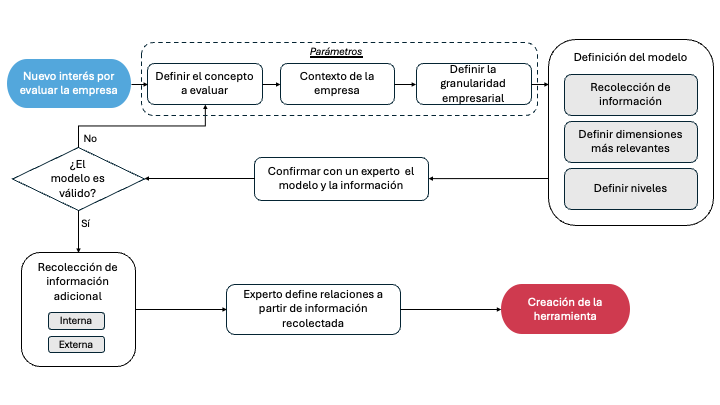
\includegraphics[scale=0.35]{images/4-desarrollo/diagrama-estrategia.png}
    \caption{Estrategia utilizada}
    \label{fig:estrategia}
\end{figure}

El segundo componente de la Figura \ref{fig:estrategia} es ‘Definición del modelo’. De este componente sale el modelo que genera la estrategia. Este es el componte se podría pensar como el más importante de todo el diagrama ya que es el producto “tangible” de la estrategia. Es en la definición del modelo donde comienza y se desarrolla la metodología explicada al principio de esta sección. En el segundo recuadro dentro de ‘Definición del modelo’, ‘Definir dimensiones más relevantes’, es donde se escoge por primera vez los KPIs previamente mencionados.  Por otro lado, ‘Definir niveles de madurez’ es el resultado de aplicar la metodología \textit{benchmarking}, es decir, el resultado de la fase ‘Recolección de información’ . También se podría considerar que el componente denominado 'Definición del modelo' es el resultado de la aplicación individual de la metodología de \textit{benchmarking} a cada subcomponente. El tercer componente del diagrama es la importancia del experto. En la sección \ref{subsec:especificaciones} \nameref{subsec:especificaciones} se habló de cómo era importante que en la herramienta generada de la estrategia no hubiera necesidad de un experto con competencias y conocimiento relacionado al concepto a evaluar (servicio ecosistémico, capital natural, especie, etc.). Sin embargo, en el desarrollo de la estrategia es imperativo la participación del experto. La participación del experto le aporta validez y robustes a la estrategia, ya que, este validará los elementos claves del modelo y la estrategia. Como se puede ver, el experto debe validar el modelo planteado y la información que fue usada y será usada más adelante. Además, el experto es quien se debe responsabilizar de hacer las conexiones entre el negocio y el ecosistema. Como se dijo en secciones anteriores, debido a que no existe una estandarización de relaciones entre elementos de un ecosistema, son los expertos basados en sus opiniones quienes deben determinar esas relaciones. El cuarto componente de este diagrama es la determinación de validez del modelo. A partir de las opiniones y sugerencias del experto, se debe aceptar o no el modelo planteado. En caso en el cual no se acepte el modelo, se debe replantear los tres parámetros a evaluar. Esto se debe a que el modelo puede estar siendo más/menos complejo de lo que en realidad debería ser con respecto al concepto, el contexto y la granularidad empresarial. También, se podría dar el caso que se deban replantear los parámetros debido a la cantidad y calidad de información disponible para la construcción del modelo. Si no hay suficiente información o la calidad de la información es de un grado menor al deseado, las conclusiones y sugerencias que llega el modelo podrán ser sesgas e inconsistentes. El componente ‘Recolección de información adicional’ hace referencia a información que aún falta recolectar sugerida por el experto para continuar con el modelo. La información interna es información relacionada a la empresa o las dimensiones que evalúa la empresa. Esto no significa necesariamente que toda la información interna deba ser de la empresa siendo evaluada. Información interna también puede ser información que un marco de referencia o guía recomienda utilizar para evaluar a una empresa. La información externa, por su parte, hace referencia a la información acerca del concepto a evaluar (ecosistema, capital natural, servicio ecosistémico, etc.) que el experto necesita para poder determinar las relaciones. Por último, la ‘Creación de la herramienta’ es el paso final de este diagrama. Esta herramienta tendrá toda la información creada y obtenida en los anteriores pasos. Por lo tanto, la herramienta será la que permita a la empresa saber su nivel con respecto al concepto que se está evaluando. 


\subsection{Recolección de información} \label{subsec:recoleccion-informacion}
La metodología de \textit{benchmarking} requiere utilizar un amplio número de fuentes de información. En el caso de este proyecto, las fuentes de información fueron utilizadas para determinar las dimensiones (\acrshort{kpis}), los niveles de madurez, los indicadores, las preguntas por dimensión que evalúan a la empresa, conceptos de evaluación, entre otras. A continuación se hará una descripción de las siete (7) fuentes de información más importantes. Existen otras fuentes de información que fueron utilizadas con un menor grado de importancia, por lo tanto, no serán explicadas a detalle. Estas fuentes de información fueron: \parencite{alliance-for-water-stewardship-2019}, \parencite{gri-2022}, \parencite{iso-1999}, \parencite{pacific-institute-2014}, \parencite{world-business-council-for-sustainable-development-2011}, \parencite{world-resources-institute-2008}, \parencite{world-wildlife-fund-2021}, \parencite{taskforce-on-nature-related-financial-disclosures-2023} y \parencite{climate-disclosure-standards-board-2022}

\subsubsection{\textit{Capital Natural Protocol}}
El \textit{Capital Natural Protocol} es un marco de referencia creado por Capital Colation que está diseñado para crear información valiosa para la toma de decisiones por parte de la altas directivas. El protocolo pretende apoyar mejores decisiones incluyendo cómo interactuamos con la naturaleza, o más específicamente con el capital natural, en la toma de decisiones \textit{\parencite{capitals-coalition-2021}}. Este documento tiene un marco de referencia divido en 4 etapas (Tabla \ref{tab:cnp-etapas}) , cada una con series de preguntas y objetivos que se deben responder y cumplir, respectivamente, para pasar a la siguiente etapa. 

\begin{table}[h!]
    \centering
    \begin{tabular}{p{3.5cm} | p{8cm} | p{3cm}}
        \centering\textbf{Etapa} & \centering\textbf{Definición}  & \textbf{Pregunta} \\
        \hline\hline
        \textit{Frame} & Identificar qué impactos de capital natural y/o dependencias son relevantes para el negocio.  & ¿Por qué?\\
        \hline
        \textit{Scope} & Establece lo que tendrá que considerar para establecer el objetivo específico para su evaluación del capital natural. & ¿Qué? \\
        \hline
        \textit{Measure and Value} & Cómo se pueden medir los impactos y las dependencias y cuál es el valor de los impactos y dependencias del capital natural. & ¿Cómo? \\
        \hline
        \textit{Apply} & Ayuda a interpretar, aplicar y actuar sobre los resultados del negocio.  & ¿Qué sigue? \\
        \hline
    \end{tabular}
    \caption{Etapas del \textit{Capital Natural Protocol} \parencite{capitals-coalition-2021}}
    \label{tab:cnp-etapas}
\end{table}

Para el desarrollo de este proyecto solo se tuvieron en cuenta las primeras etapas, ya que la cuarta etapa menciona futuros cambios y acciones, lo cuales no fueron contemplados ya que están asociados a las oportunidades y riesgos. El protocolo se basa en los siguientes cuatro (4) principios: relevancia, la cual busca que la empresa este considerando los problemas o circunstancias realmente más importantes; rigor, la información y los datos utilizados deben venir de perspectivas científicas o económicas; replicabilidad, todos los supuestos, datos y métodos utilizados son transparentes, documentados y repetibles; y, por último, consistencia, los datos y métodos utilizados durante el uso del marco de referencia son compatibles entre ellos, además de depender de los objetivos y expectativas de la aplicación del marco de referencia \parencite{capitals-coalition-2021}.



\subsubsection{ISO 14001 e ISO 14004}
Las normas de la Organización Internacional de Normalización (ISO) son utilizadas como marcos de referencias que ayudan a diferentes organizamos en diferentes contextos a lograr algún objetivo basándose en una estructura y estándares específicos. La norma ISO 14001 denominada “Sistemas de Gestión Ambiental – Requisitos con orientación para su uso” \parencite{iso-2015} fue la fuente principal para determinar las dimensiones (KPIs) que serían evaluadas para determinar el nivel de la empresa. En la sección \ref{sec:implementacion}. \nameref{sec:implementacion} se entra en mayor detalle de cómo se utilizó cada una de las dimensiones. Sin embargo, debido al objetivo de la ISO 14001, se considera que cada sección de la guía contempla las dimensiones clave que deben tenerse en cuenta al evaluar una empresa. El objetivo, según la guía \textcite{iso-2015}, es

\hfill
\par
\leftskip=0.35in \rightskip=0.35in
Esta Norma Internacional especifica los requisitos de un sistema de gestión ambiental para organizaciones que buscan establecer, implementar, mantener y mejorar continuamente un marco de referencia con el fin de gestionar sus responsabilidades ambientales de una forma que contribuya al “pilar ambiental” de la sostenibilidad.

\hfill
\par
\leftskip=0in \rightskip=0in
Por otro lado, la norma  ISO 14004 denominada “Sistemas de gestión ambiental – Directrices generales sobre principios, sistemas y técnicas de apoyo” \parencite{iso-2004} fue utilizada principalmente para evaluar la dimensión de Soporte. Es decir, la norma ISO 14004 fue utilizada para evaluar la empresa en sector de capital humano, específicamente, en los recursos, educación y comunicación brindada a los trabajadores dentro de la empresa. La razón principal de haber utilizado esta guía para evaluar dicha dimensión se debe a la justificación que presenta la misma norma. 

\hfill
\par
\leftskip=0.35in \rightskip=0.35in
Facilitar informaci\'on apropiada a los empleados de una organizaci\'on sirve para motivarlos y para fomentar la aceptaci\'on de los esfuerzos de la organizaci\'on para mejorar su desempe\~no ambiental. Esto puede ayudar a los empleados a cumplir sus responsabilidades y a la organizaci\'on a cumplir sus objetivos y metas ambientales. La organizaci\'on deber\'ia contar con un proceso para fomentar la retroalimentaci\'on y el compromiso de todos los niveles de la organizaci\'on, y recibir y responder las sugerencias e inquietudes de los empleados \parencite{iso-2004}. 

\hfill
\par
\leftskip=0in \rightskip=0in

El extracto anterior se considera que está alineado con las importancias ya mencionadas en la sección \ref{subsec:identificacion-problema-importancia}. \nameref{subsec:identificacion-problema-importancia}. La estrategia que se busca implementar dentro de este documento considera que la participación de todos los trabajadores involucrados dentro de la empresa debe ser actores activos. La mejora, el cambio y el progreso hacia un mejor nivel debe estar acompañado por un alineamiento unánime de todos los actores dentro de la empresa. 

\subsubsection{GRI 303: Agua y efluentes 2018}

La “GRI 303: Agua y efluentes 2018 incluye contenidos para que las organizaciones presenten información acerca de sus impactos relacionados con el agua y la manera en que gestionan estos impactos” \parencite{gri-2019}. La guía GRI 303 hace parte de los estándares GRI, los cuales, tienen como objetivo informar de la mejor manera a una empresa, ente gubernamental o grupo de personas específicas acerca de un impacto económico, ambiental o social.  La guía GRI 303 fue utilizada debido a que presenta información valiosa que una empresa debería tener en cuenta cuando trata con agua. El documento presenta tres secciones que solicitan a una empresa, que desee seguir el estándar, documentar y medir. La extracción del agua, el vertido del agua y el consumo del agua son tres componentes que una empresa debe medir y documentar para determinar el impacto sobre ecosistemas relacionados con el agua. Estos tres componentes fueron tenidos en cuenta a la hora de desarrollar la herramienta, ya que en la etapa de indicadores, se evalúan estos tres componentes.


\subsubsection{SASB}
Los estándares SASB tienen por objeto ayudar a las entidades a revelar información sobre los riesgos y oportunidades relacionados con la sostenibilidad que razonablemente podrían afectar a los flujos de efectivo de la entidad, su acceso a la financiación o el coste del capital a corto, medio o largo plazo \parencite{sasb-standards-2023}. Debido al reconocimiento global de este estándar, a la facilidad de uso de su página web y al consejo del experto, se decidió utilizar la clasificación de sectores e industrias proporcionada por dicho estándar. Este estándar también presenta un amplio repertorio de indicadores relacionados a diversos capitales naturales que fueron utilizados para relacionar a la empresa con los ecosistemas.  


\subsubsection{Manual de Estrategias para la Naturaleza}
Según \textcite{its-now-for-nature-2023} en su  “Manual de Estrategias para la Naturaleza”,

\hfill
\par
\leftskip=0.35in \rightskip=0.35in
El objetivo del Manual de Estrategias para la Naturaleza es apoyar a todas las empresas, ya sean corporaciones o instituciones financieras, en el desarrollo de una estrategia para la naturaleza que les permita contribuir significativamente a un mundo positivo para la naturaleza.

\hfill
\par
\leftskip=0in \rightskip=0in
El manual utilizada la metodología Evaluar, Comprometerse, Transformar y Divulgar (ACT-D) \parencite{its-now-for-nature-2023}, la cual guía a las empresas a través de diferentes herramientas y les ayuda, también, a fijar objetivos relacionados a disminuir el impacto en la naturaleza. Este manual es de gran importancia para el desarrollo de este documento y la generación de preguntas en la implementación de la herramienta. El Manual de Estrategias para la Naturaleza, fue utilizado como corroboración y revisión de preguntas en el paso de Cuestionario en el despliegue de la aplicación web (\ref{subsec:implementacion-desarrollo-herramienta}. \nameref{subsec:implementacion-desarrollo-herramienta}). 


\subsubsection{\textit{CDP Water Security 2023 Questionnaire}}

Esta fuente de información fue la fuente principal para el desarrollo del cuestionario de la aplicación web. El cuestionario de agua ayuda a las empresas a impulsar mejoras en la gestión del agua y permite la comparación con las prácticas líderes \parencite{disclosure-insight-action-2023}. Aunque en el documento se establece que el cuestionario está orientado a riesgos y oportunidades, muchas de las preguntas incluidas están relacionadas con las dependencias e impactos. El cuestionario está dividido en diez (10) secciones diferentes, las cuales buscan evaluar cada dimensión de una empresa para determinar los riesgos y oportunidades posibles. Estas diez (10) dimensiones no fueron escogidas sobre las proporcionadas por la ISO 14001, ya que las dimensiones del \textcite{disclosure-insight-action-2023} están orientadas a riesgos y oportunidades en lugar de dependencias e impactos. Además, no todas las dimensiones de este cuestionario se consideran relevantes, mientras que todas las dimensiones de la ISO 14001 sí se consideran vitales para la evaluación de la empresa. Según \textcite{disclosure-insight-action-2023}, existen 85 preguntas sin incluir preguntas específicas por sector o de cadena de suministro. Esto se debe a que el camino que toma cada empresa será diferente dependiendo no solo de su sector, sino respuestas en diferentes dimensiones que desencadenan preguntas específicas.

\subsection{Alternativas de diseño} \label{subsec:alternativas-diseno}
La Figura \ref{fig:estrategia} muestra cuál fue la manera genérica que se evaluó cada estrategia considerada. En esta sección se explicará las dos estrategias que se plantearon que no fueron escogidas. Se explicará el objetivo principal de la estrategia, los parámetros considerados, el modelo desarrollado y las razones por las cuales no fue escogida. 

\subsubsection{Estrategia: Primer acercamiento}
La estrategia 'Primer acercamiento' fue la primera estrategia que fue planteada y analizada para este proyecto. Como se puede ver en la Figura \ref{fig:primer-acercamiento} la estrategia incluye cuatro pasos principales, no incluye un modelo explícitamente y de los parámetros solo es tomado en cuenta el contexto de la organización. El objetivo principal de esta estrategia era proporcionarle información extra a la empresa según el estado actual de la misma. En el primer paso, y único parámetro tenido en cuenta, se buscaba comprender el contexto de la organización. En este paso se busca obtener la información geográfica de la empresa, su sector e industria, y por cada servicio ecosistémico que la empresa usara sus dependencias, impactos, riesgos y oportunidades. En este paso ya se pueden ver varios inconvenientes. El primero es la falta de información adicional que no se le pedía a la empresa. Al solo pedirle la ubicación geográfica o su sector e industria se estaban incurriendo en los mismos problemas que las herramientas \nameref{subsubsec:encore} y \nameref{subsubsec:wwf-water-risk-filter}. Adicionalmente, se estaba haciendo un supuesto bastante flexible y errónea en cual consistía que las empresas sabían desde un principio todos los \acrshort{ssee} de los cuales dependerían, impactaban, tenían riesgos y oportunidades. Entonces, bajo este supuesto, el objetivo de esta estrategia se perdía ya que, si la empresa no sabía nada, se le tendría que mostrar toda la información disponible en la herramienta. El problema de lo anterior es que si se le muestra toda la información disponible cuando la empresa desde un principio no tiene información, es muy probable que esta no vaya a saber cómo utilizarla, aprovecharla y aplicarla.

\begin{figure}[h!]
    \centering
    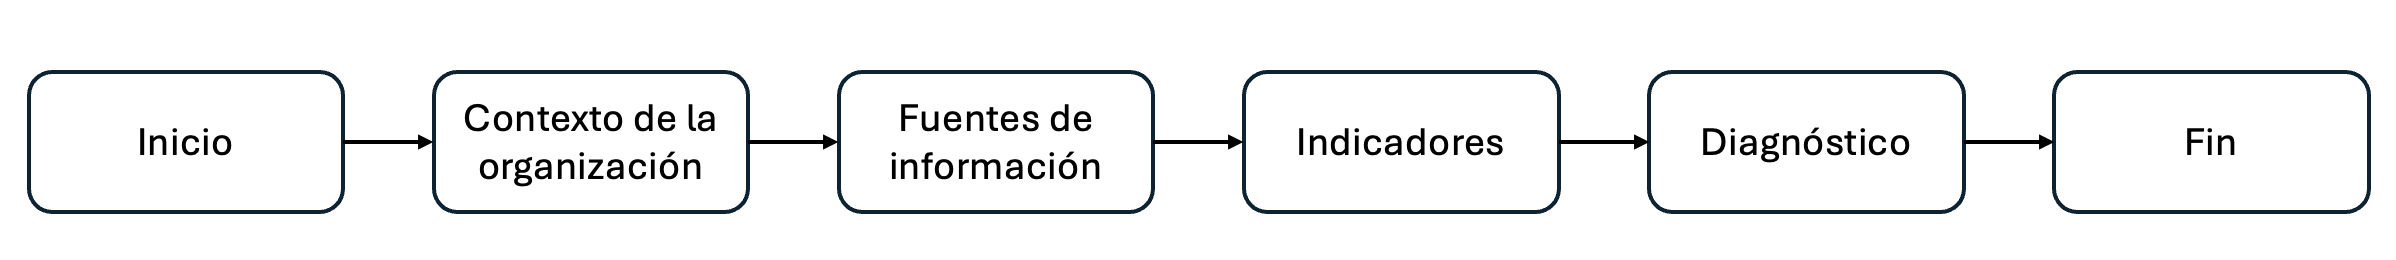
\includegraphics[scale=0.35]{images/4-desarrollo/estrategia-primer-acercamiento.png}
    \caption{Primer acercamiento}
    \label{fig:primer-acercamiento}
\end{figure}

El siguiente paso en la Figura \ref{fig:primer-acercamiento} denominado ‘Fuentes de información’ consistía en obtener las fuentes de información que la empresa utilizaba. Este paso sufría el mismo problema que el paso anterior. Cuando la empresa no tenía información este paso no se podría aplicar, es decir, el 25\% de la estrategia sería inutilizable. Cuando la empresa si tenía información, la intención de este paso era analizar y evaluar dicha información. Evaluar su temporalidad, rigurosidad, confiabilidad, utilidad, granularidad, comparabilidad, etc. A partir de estas dimensiones, se le mostraría a la empresa su nivel con respecto a la información que utiliza. 

El propósito del tercer paso, ‘Indicadores’, dependía directamente de los anteriores dos pasos. La intención era mostrarle a la empresa los indicadores que existían según la información que esta tenía. Entonces, si la empresa no tenía información, no se podía evaluar y adicionalmente, no se le podía mostrar indicadores. Por lo tanto, se estaría perdiendo 50\% de la estrategia. Se podría pensar en el caso que la empresa no tenga nada de información mostrarle toda la disponible más todos los indicadores disponibles, pero se estaría cayendo en una trampa. Si se le muestra toda la información y sus indicadores respectivos sin ninguna asistencia o guía, la empresa no sabría que hacer con ella. Este paso, por otro lado, no contemplaba el hecho que las empresas podían estar midiendo indicadores adicionales a los disponibles. Esto perjudicaba a la empresa ya que no le permitía analizar sus indicadores actuales. 

Finalmente, en el último paso, ‘Diagnóstico’, se busca mostrar un nivel de madurez con respecto a los tres anteriores pasos. Es decir, a partir de la información obtenida en el contexto de la organización y la evaluación de lo información que dispone la empresa, se determinaba un nivel de madurez. En el momento que se estaba desarrollando esta estrategia nunca se llegó a pensar en sus KPIs, lo cual, es otro indicio porque esta estrategia no fue aplicada. En conclusión, esta estrategia no fue aplicada debido a la alta dependencia entre cada etapa, la falta de rigurosidad y la generalización de las empresas. Además, no mostraba indicios de concienciar a las empresas para realizar cambios hacia el cuidado y la sostenibilidad de los ecosistemas. Finalmente, la estrategia no contemplaba la ayuda u opinión de expertos, y como ya se explicó en secciones anteriores, a opinión y conocimientos de estos es muy importante en el contexto de los ecosistemas y sus componentes. 

\subsubsection{Matriz de dimensiones} \label{subsubsec:matriz-dimensiones}
La segunda estrategia que fue tomada en cuenta se llamó Matriz de dimensiones. En la Figura \ref{fig:estrategia-matriz-dimensiones} se puede observar la estrategia que se llevó a cabo. Esta estrategia busca determinar el nivel de una empresa contemplando todos los \acrshort{ssee} de la cual esta dependía e impactaba. A pesar de que esta estrategia estaba dirigida a una empresa genérica, la granularidad empresarial era un proceso específico de la empresa. Entonces, el objetivo de esta estrategia era determinar el nivel de madurez de una empresa según las dependencias e impactos que tenía sobre todos los \acrshort{ssee} que utilizase en un proceso en específico.

\begin{figure}[h!]
    \centering
    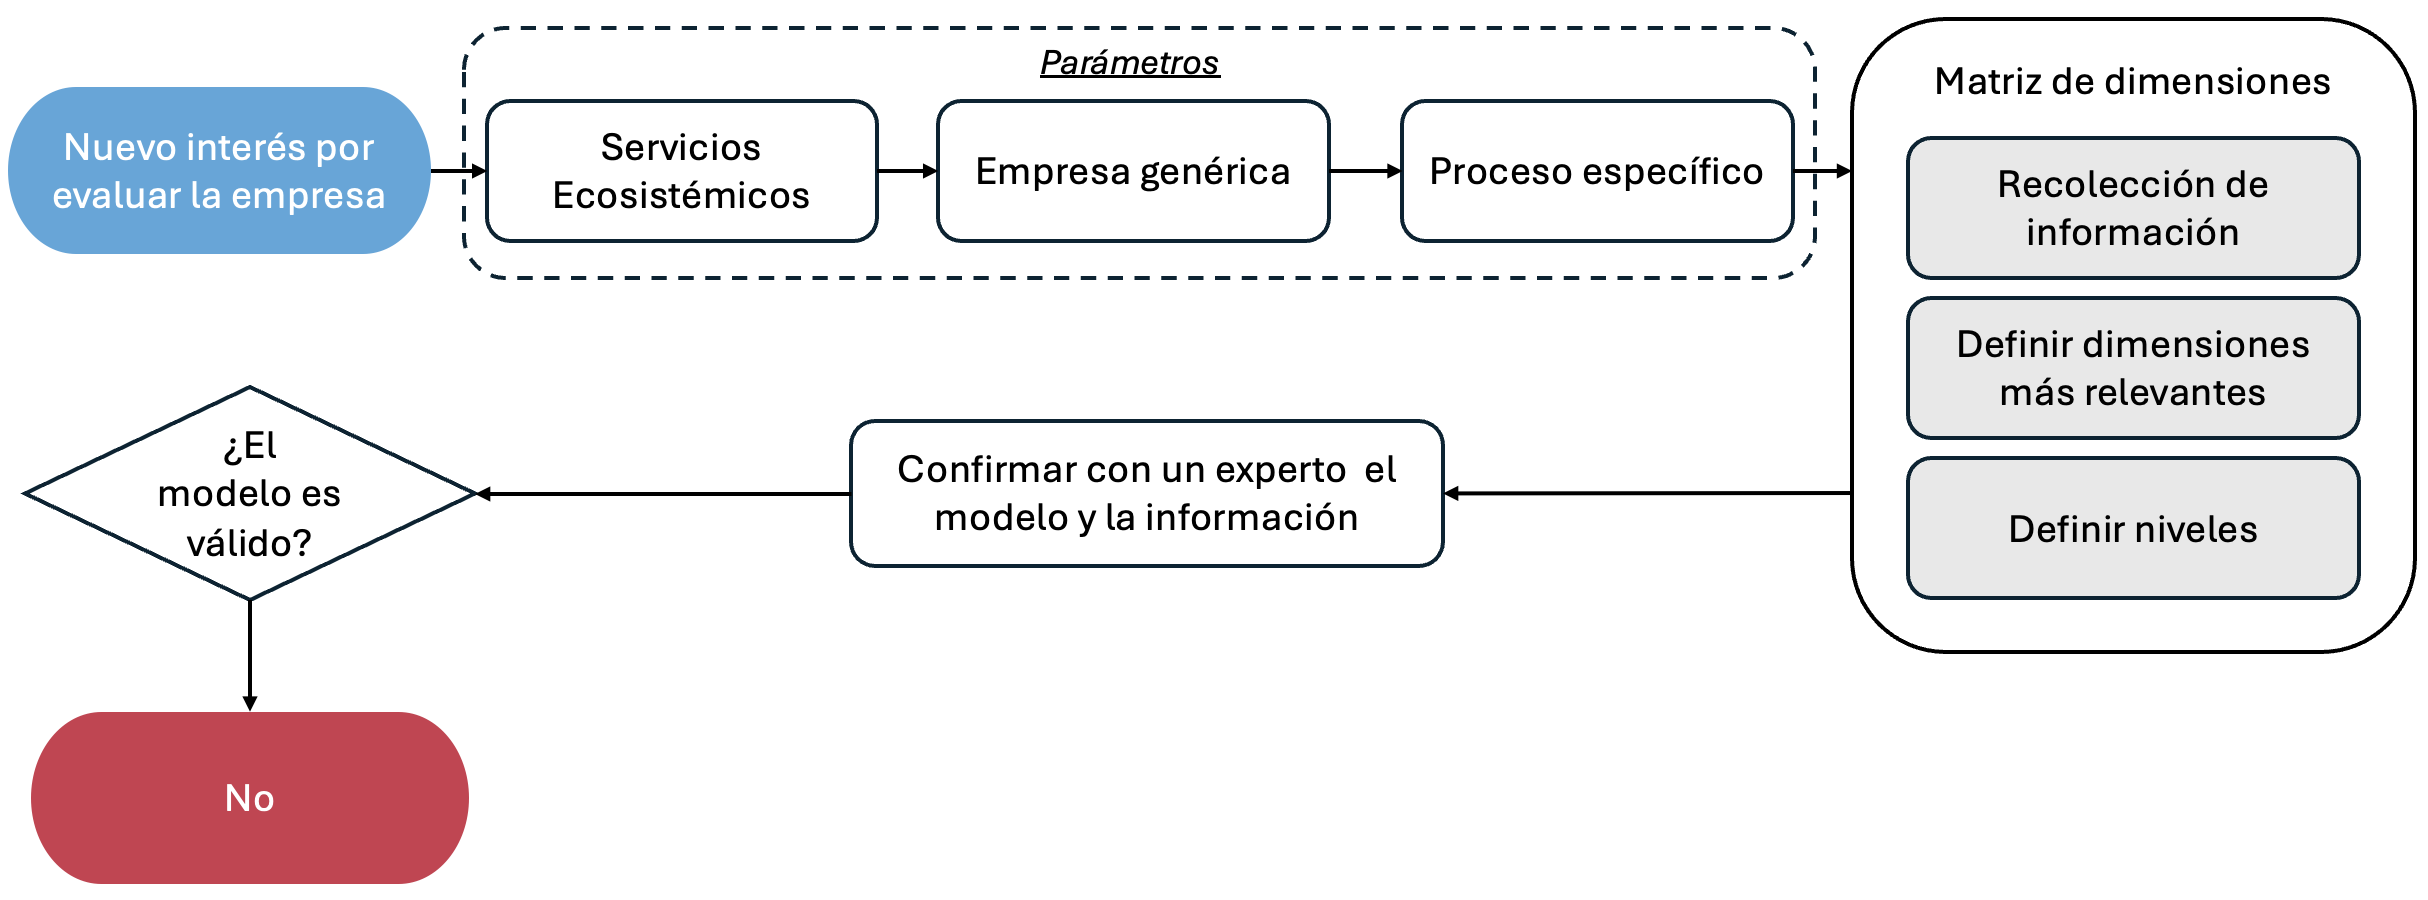
\includegraphics[scale=0.35]{images/4-desarrollo/estrategia-matriz-dimensiones.png}
    \caption{Diagrama de la estrategia Matriz de dimensiones}
    \label{fig:estrategia-matriz-dimensiones}
\end{figure}

En la Figura \ref{fig:proceso-matriz-dimensiones} se muestra el paso que se debía hacer antes de implementar la estrategia. En este paso se determinaba cuál proceso de la empresa se evaluaría. Primero, se escogían todos los procesos candidatos de la empresa. Según los objetivos del negocio, la factibilidad de cambio, los dolores que generaban no tener el proceso evaluado, las necesidades que surgían del proceso y las oportunidades que tiene el proceso se graficaba el proceso. Teniendo en cuentas todas las anteriores variables, se determinaba el impacto y la factibilidad, es decir, cuál es el impacto tanto a nivel empresarial como ecosistémico de cambiar el proceso versus cuál es la factibilidad de ese cambio. El proceso que tuviera el mayor impacto y la mayor factibilidad era el escogido para ser evaluado.  

\begin{figure}[H]
    \centering
    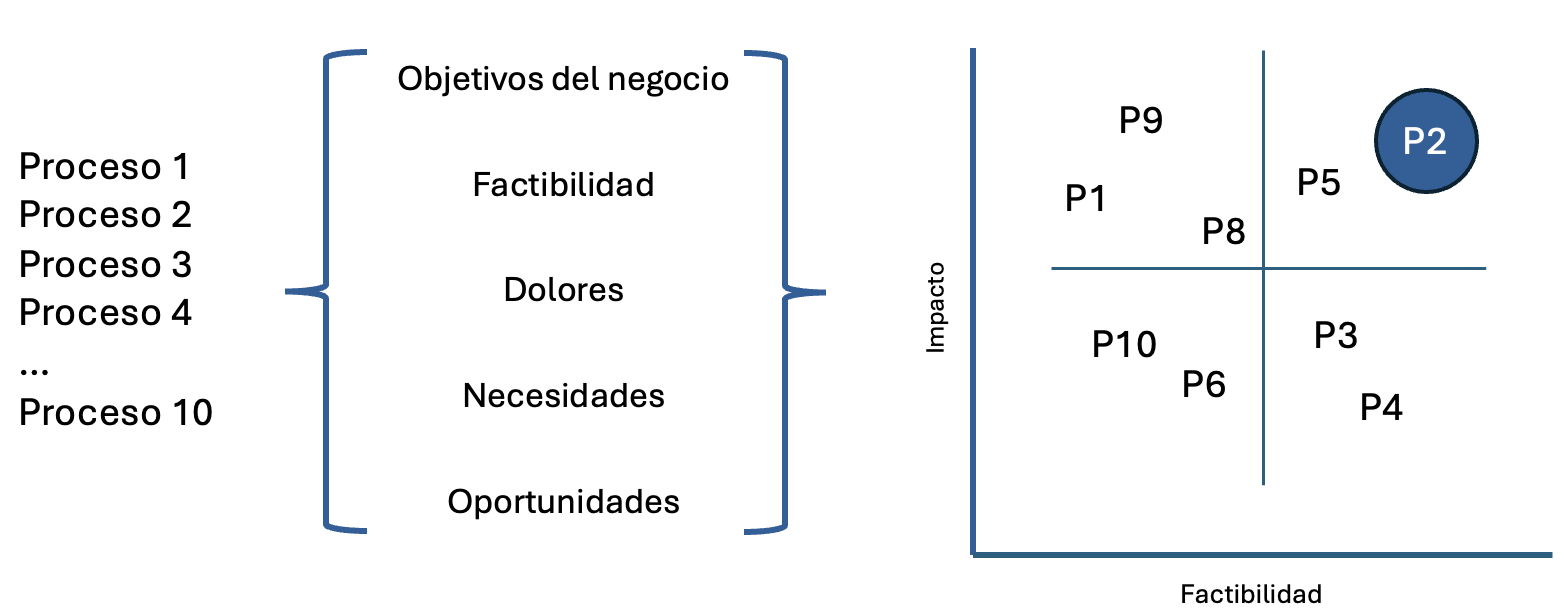
\includegraphics[scale=0.45]{images/4-desarrollo/proceso-matriz-dimensiones.png}
    \caption{Etapas para escoger el proceso en la estrategia Matriz de dimensiones}
    \label{fig:proceso-matriz-dimensiones}
\end{figure}

Cuando ya se hubiera escogido el proceso se procedía a evaluarlo. Esta evaluación se hacía a partir de modelo escogido en esta estrategia denominado Matriz de dimensiones \ref{fig:matriz-dimensiones}. Este modelo buscaba evaluar el proceso en cada una de las dimensiones que se ven en el diagrama. Por cada dimensión se le otorgaba un nivel, siendo uno (1) el peor nivel y cinco (5) el mejor. Luego de tener el nivel para cada dimensión, se determinaba el nivel general del proceso. En la Tabla \ref{tab:matriz-dimensiones} se puede ver la descripción de cada dimensión que evaluaba al proceso.

\begin{figure}[H]
    \centering
    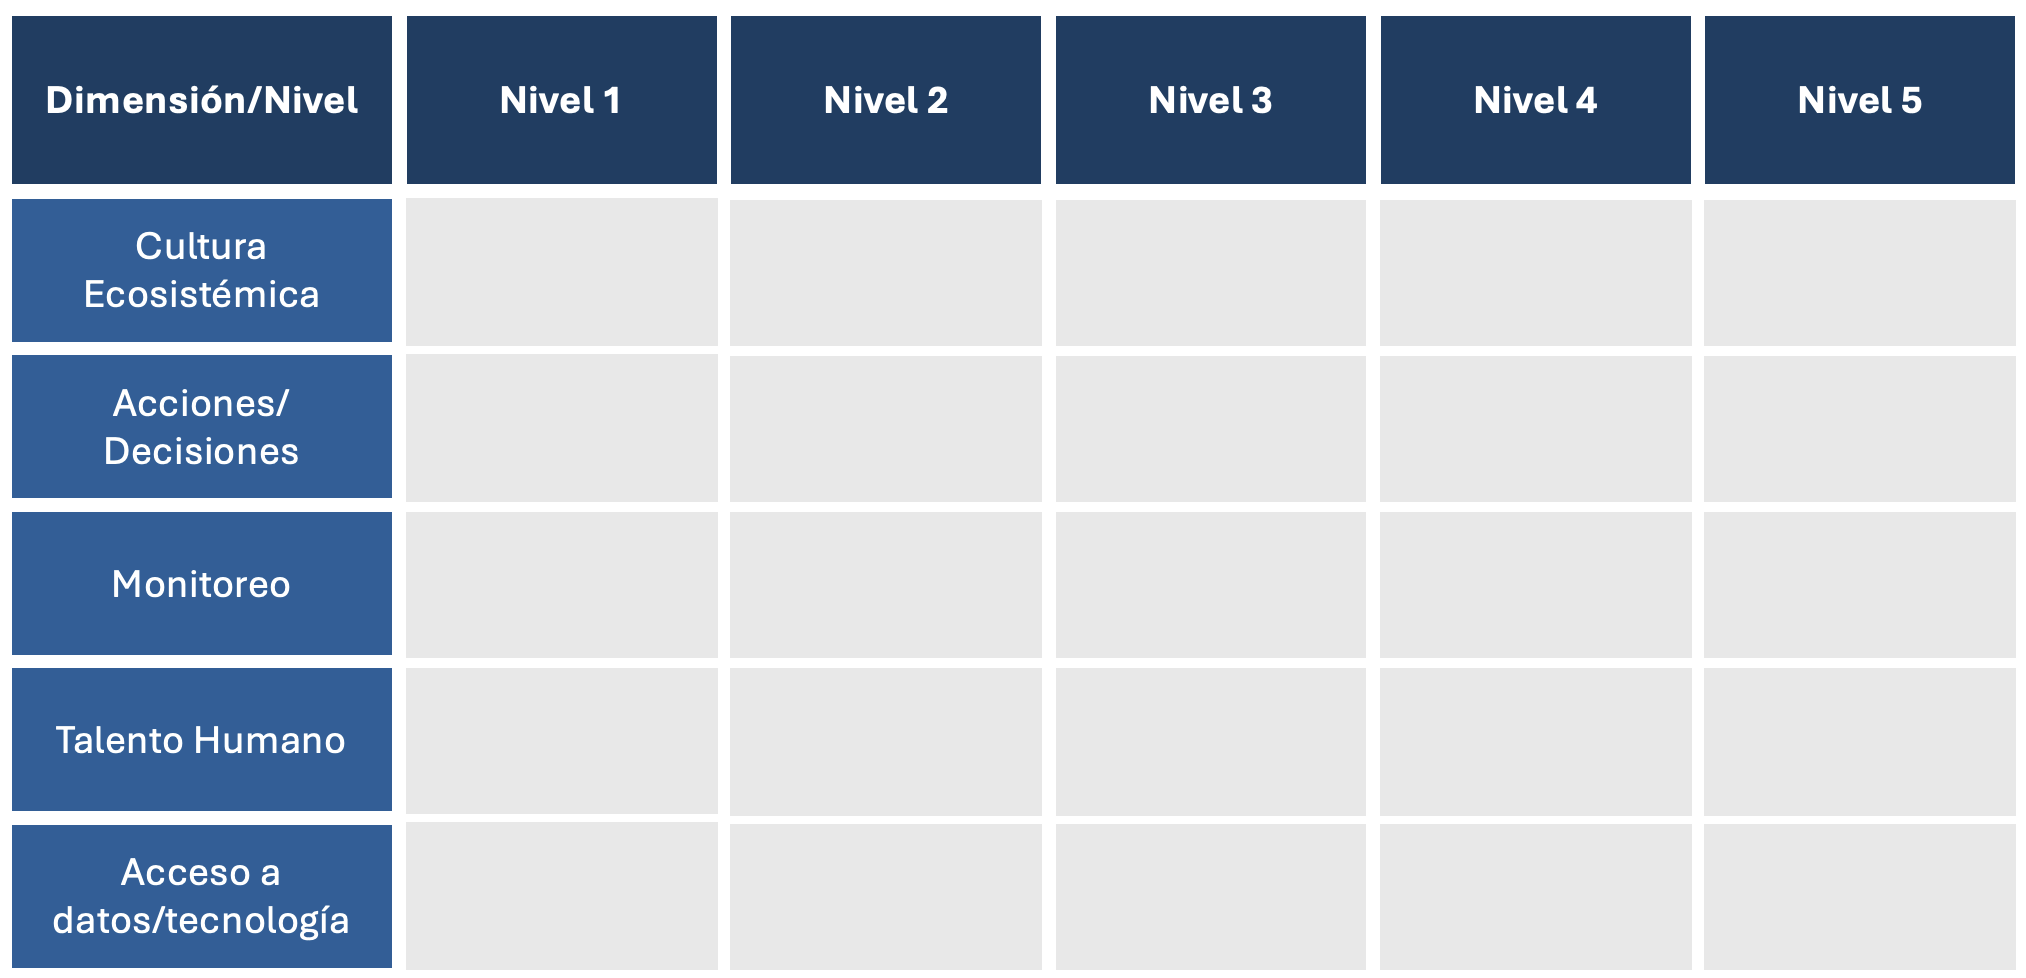
\includegraphics[scale=0.4]{images/4-desarrollo/matriz-dimensiones.png}
    \caption{Matriz de dimensiones}
    \label{fig:matriz-dimensiones}
\end{figure}


\begin{table}[H]
    \centering
    \begin{tabular}{p{5cm} | p{10cm}}
        \textbf{Dimensión} & \textbf{Descripción} \\
        \hline\hline
        Cultura Ecosistémica & Conocimiento y comprensión que tiene una empresa sobre su relación con los ecosistemas, incluyendo sus dependencias, impactos y el contexto ecosistémico de sus procesos.\\
        \hline
        Acciones/ Decisiones & El concepto de SSEE hace parte de la toma de decisiones y acciones hechas en el proceso.\\
        \hline
        Monitoreo & Seguimiento regular y evaluaciones periódicas de la relación entre un proceso y el ecosistema, incluyendo sus costos en términos de dinero, tiempo y mano de obra.\\
        \hline
        Talento Humano & Calidad del conjunto de personas, tanto internas como externas, involucradas en un proceso. \\
        \hline
        Acceso a datos/tecnología & Disponibilidad, facilidad de obtención y uso de datos y tecnologías para la recolección y análisis de información en un proceso.\\
        \hline
    \end{tabular}
    \caption{Explicación de dimensiones en Matriz de dimensiones}
    \label{tab:matriz-dimensiones}
\end{table}

El principal problema de la estrategia Matriz de dimensiones era la falta de información rigurosa o estandarizada para responder la pregunta “¿Qué significa ser nivel X para la dimensión Y?”.  Debido que calificar al proceso dependía del nivel por dimensión, la respuesta a la anterior pregunta debía tener un soporte, formalidad, estandarización y rigurosidad que actualmente no existe. Como bien se ha dicho en este documento, la opinión de los expertos es vital para cualquier estrategia debido a la falta de estandarización en el campo. Sin embargo, basar todo el modelo en la opinión de expertos es ir al extremo radical, el cual es un error. Cuando determinar qué significa ser nivel X en la dimensión Y para cada nivel por cada dimensión basándose en la opinión del experto, es más que probable que el modelo vaya a ser sesgado e inconsistente. No solo por la falta de información, sino porque no hay unanimidad en el contexto de los ecosistemas para aceptar 25 calificaciones (5 dimensiones x 5 niveles).

El segundo problema, algo relacionado con el primero, era la falta de formalidad que tenía la escogencia de las dimensiones. Las dimensiones presentadas en la matriz no vienen de ningún marco de referencia, manual, guía o estándar ya existente. Esto genera que exista posibles confusiones ya que a pesar de que se pueda definir la dimensión, no existe una fuente confiable que expanda sobre esta. Esto quiere decir, que el modelo no solo puede llegar a confundir, sino que también es necesario hacer una extensión por cada dimensión escogida. Explicarla detalladamente, justificar por qué no se escogieron más y por qué es suficiente solo estas dimensiones son las preguntas que se deberían responder.  El ejercicio anterior se podría hacer, el inconveniente es que no existe un respaldo oficial sobre este. En cambio, todos los componentes de la estrategia escogida en este documento fueron basados en marcos de referencia, manuales, guías o estándares ya existente. Esto le da validez, formalidad y soporte a la estrategia, algo que no es posible para la estrategia Matriz de dimensiones.

